\documentclass[11pt]{article}
\usepackage{latexsym}
\usepackage{amsmath}
\usepackage{amssymb}
\usepackage{amsthm}
\usepackage{epsfig}
\usepackage[tight]{subfigure}
\usepackage{cases}
\usepackage{amsmath}

\DeclareMathOperator*{\minimize}{min}
\DeclareMathOperator*{\maximize}{max}

\usepackage{algorithm}
 %on linux you may need to run sudo apt-get install texlive-full to install algorithm.sys
\usepackage{algorithmic}

\usepackage{verbatim}

\newcommand{\handout}[5]{
  \noindent
  \begin{center}
  \framebox{
    \vbox{
      \hbox to 5.78in { {#1} \hfill #2 }
      \vspace{4mm}
      \hbox to 5.78in { {\Large \hfill #5  \hfill} }
      \vspace{2mm}
      \hbox to 5.78in { {\em #3 \hfill #4} }
    }
  }
  \end{center}
  \vspace*{4mm}
}

\newcommand{\lecture}[5]{\handout{#1}{#2}{#3}{#4}{#5}}
\newcommand{\collision}[0]{\mathrm{collision}}
\newcommand{\nocollision}[0]{\overline{\collision}}

\newcommand*{\QED}{\hfill\ensuremath{\square}}

\newtheorem{theorem}{Theorem}
\newtheorem{corollary}[theorem]{Corollary}
\newtheorem{lemma}[theorem]{Lemma}
\newtheorem{observation}[theorem]{Observation}
\newtheorem{proposition}[theorem]{Proposition}
\newtheorem{definition}[theorem]{Definition}
\newtheorem{claim}[theorem]{Claim}
\newtheorem{fact}[theorem]{Fact}
\newtheorem{assumption}[theorem]{Assumption}
\newtheorem{note}[theorem]{Note}

% 1-inch margins, from fullpage.sty by H.Partl, Version 2, Dec. 15, 1988.
\topmargin 0pt
\advance \topmargin by -\headheight
\advance \topmargin by -\headsep
\textheight 8.9in
\oddsidemargin 0pt
\evensidemargin \oddsidemargin
\marginparwidth 0.5in
\textwidth 6.5in

\parindent 0in
\parskip 1.5ex
%\renewcommand{\baselinestretch}{1.25}

\begin{document}

\lecture{Statistical Techniques in Robotics (16-831, S22)}{Lecture \#11
  (Wednesday, February 23)}{Lecturer: Kris Kitani}{Scribes: Meghdeep Jana, Moneish Kumar}{AdaBoost \& Multi-Arm Bandits}

\section{Review}
In the last lecture, we learned about an online supervised learning algorithm, Online Support Vector Machine(SVM). As discussed in the lecture, we review two variations of SVM below.

%This section serves as a review of the previous lecture and any other context required to frame the content of the current lecture. 

%You may format the scribes in any way you like, aside from changing font style, size and page format. Please use subsections and paragraphs to increase the readability of your notes.

%Length requirement 1-2 pages.
        
\subsection{Max-Margin and Hard SVM}
Support Vector Machines (SVMs)\cite{svm} aims to find a hyperplane (decision boundary) in the feature space that separates the closest points of two different classes by as maximum distance as possible. This distance between the two extreme ends of hyperplane is called as margin (Shown in fig \ref{fig:svm}. More formally, let's say the hyperplane is:

\begin{figure}[h!]
    \centering
    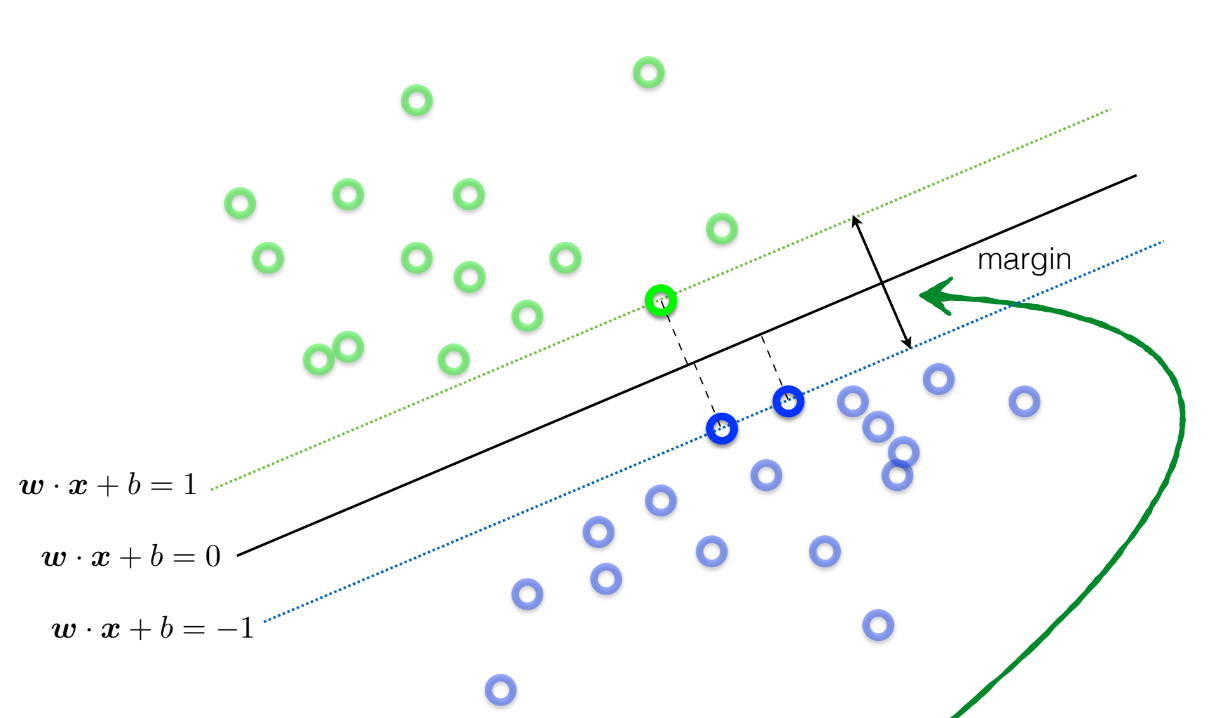
\includegraphics[width=0.75\linewidth]{images/svm.png}
    \caption{Max-Margin formulation of SVM. It tries to find a hyperplane that maximizes the distance between data points of two different classes}
    \label{fig:svm}
\end{figure}


\begin{equation}
    w.x + b =0 
\end{equation}

For two class setting the objective of SVM can be formulated as a maximization problem:

\begin{numcases}
{max_{\mathbf{w}} \frac{2}{||\mathbf{w}||}, \quad s.t. \quad \mathbf{w} \cdot \mathbf{x}_i + b \quad}
      \geq +1  \text{ if } y_i = +1 \\
      \leq -1 \text{ if } y_i = -1 .
\end{numcases} 

Its form as a minimization problem would be:

\begin{equation}
    min_{\mathbf{w}} || \mathbf{w} ||^2, \quad s.t. \quad y_i (\mathbf{w} \cdot \mathbf{x}_i + b ) \geq 1  ( i = 1,..., N),
\end{equation}

The above optimization problem can be solved using quadratic programming. The above formulation is known as "Hard-SVM" and assumes that the data is linearly separable. Further, we introduce a variant of SVMs that relaxes this assumption.

\subsection{Soft SVM and Sub-gradients}
The Hard SVM, as seen above tries to classify all labels correctly. This works only in the case of linearly separable data, also if we consider that usually data has some inherent noise and we would want to create a robust model that is not affected by such noise. This is achieved by soft SVM wherein we accept some classifications to create an SVM with a larger margin i.e that this SVM is more robust or has a lower variance. For each data point $x_i$ we would want the following condition to hold.
\begin{align}
    y_i(w^Tx_i + b) \ge 1 - \xi_i \; \forall \; i
\end{align}
Here $\xi_i$ is called the slack variable. The objective function now becomes:
\begin{align}
    \minimize_{w,\xi_i} ||w||^2 + C \sum_{i}\xi_i
\end{align}
Combining both equations we get our final objective function:
\begin{align}
    \minimize_{w} \frac{\lambda}{2}||w||^2 + \frac{1}{M} \sum_{i=0}^{M}\max(0, 1 - y_iw^Tx_i)
\end{align}
The above objective function is convex but is not differentiable because of the second part (hinge loss). This optimisation is solved using sub-gradient descent. A sub gradient of a convex function f(x) where x $\in\; \mathbb{R}^n$ is g $\in \; \mathbb{R}^n$ such that:
\begin{align}
    f(y) \ge f(x) + g^T(y-x)
\end{align}
For Hinge Loss the subgradients are:
\begin{align}
    gi = \begin{cases}
    0 & y_iw^tx_i \geq 1 \\
    -y_iw^tx_i  & otherwise
    \end{cases}
\end{align}
The algorithm for soft SVM with subgradient descent is as follows:

\begin{algorithm}[H]
\caption{Soft SVM}
\label{algo:soft-svm}
\begin{algorithmic}[1]
\STATE $\boldsymbol{\theta}^{(1)} \leftarrow \mathbf{0} \in \mathbb{R}^N$
\FOR{$t=1,\;\cdots,\;T$}
\STATE $y_i, \boldsymbol{x}_i \sim \boldsymbol{D}$
\STATE $\boldsymbol{\theta}^{(t)} = \boldsymbol{\theta}^{(t-1)} + y_i \boldsymbol{x}_i \cdot \mathbf{1} [y_i (\boldsymbol{w}^{(t)} \cdot \boldsymbol{x}_i) < 1]$
\STATE $\boldsymbol{w}^{(t+1)} \leftarrow \frac{1}{\lambda(t+1)} \boldsymbol{\theta}^{(t)}$
\ENDFOR
\end{algorithmic}
\end{algorithm}
\section{Summary}



\subsection{Probably Approximately Correct(PAC) Learning}
\normalfont

Probably Approximates Correct(PAC) learning is a theoretical framework that tries to answer the following two questions:
\begin{itemize}
\item What is the optimal dataset size to obtain good generalization?
\item What is the computational cost of learning?
\end{itemize}

Let's consider a dataset $\mathcal{D}$ of size $N$ that is drawn from an underlying distribution $P(x,y)$. Here, the class labels are determined by an unknown deterministic distribution $y=f^*(x)$ this can be called as the "perfect hypothesis" in online learning domain. The dataset $\mathcal{D} \text{ forms } \Tilde{P}(x,y) $ which is an approximation of true distribution $P(x,y)$ and more samples we draw, the better is the approximation. 

We define a space of functions $\mathcal{F}$ (hypothesis class) containing functions defined on the basis of the training set $\mathcal{D}$. We then define a function $f(x;\mathcal{D})$ drawn from $\mathcal{F}$ that can be thought of as a classifier learned from the training data. A function $f(x)$ has good \textbf{generalization} if its expected error rate is less than a pre-defined threshold parameter $\epsilon$. This can be expressed as:

\begin{equation}
    \mathbb{E}_{P(x, y)}[\mathbf{1}[f(x; \mathcal{D}) \neq y]] < \epsilon
    \label{eqn:gen}
\end{equation}

We can now define the PAC learning algorithm. It is a learning algorithm that requires \eqref{eqn:gen} to hold with a probability of $(1-\delta)$ for any dataset $\mathcal{D}$ drawn from $P(x,y)$. Here, $\delta$ is a pre-defined value. There are two types of PAC learning algorithms:

\definition{\textbf{Strong PAC Learner} This PAC learning algorithm outputs with a probability $(1-\delta)$ a hypothesis function $f(x)$ with error at most $\epsilon$.}

\definition{\textbf{Weak PAC Learner} This PAC learning algorithm outputs with a probability $(1-\delta)$ a hypothesis function $f(x)$ with error at most $\epsilon \geq \frac{1}{2}- \gamma$. Here, $\gamma>0$.}
\normalfont

For both strong and weak PAC-learning algorithms, the run time must to polynomial in $1/\delta$ and $1/\epsilon$ and other relevant parameters such as the size of the examples or complexity of the target concept.

Boosting is a strategy where an ensemble of weak learners are presented with a different distribution $\mathcal{D}$ and their hypothesis are combined into a single hypothesis which is the strong learner \cite{hyp_boosting}. The key idea here is that any weak learning algorithm can be boosted into a strong learning algorithm \cite{boosting}. PAC learning makes the connection between boosting and online learning. Further, we introduce a learning algorithm that leverages this concept of boosting.

\subsection{AdaBoost}

We introduce Adaptive Boosting (AdaBoost), which is a machine learning that is used in conjunction with many other types of learning algorithms to improve performance. The output of the other learning algorithms ('weak learners') is combined into a weighted sum that represents the final output of the boosted classifier\cite{wiki_adap}. The Adaboost algorithm is shown in Algorithm \ref{algo:adaboost}. 

\begin{algorithm}[H]
\caption{AdaBoost\cite{adaboost}}
\label{algo:adaboost}
\begin{algorithmic}[1]
\REQUIRE $D=\{x_n, y_n\}_{n=1}^N$, $\{w_n^{(0)}\}_{n=1}^N$, $T$
\FOR{t=1,...,T }
\STATE $\mathbf{p}^{(t)} = \mathbf{w}^{(t-1)} / \sum_{n} w_n^{(t-1)}$
\STATE $h^{(t)} = $ WEAKLEARNER $(D, \mathbf{p}^{(t)})$
\STATE $\epsilon^{(t)} = \sum_n p_n^t | h^{(t)} (x_n) - y_n | $
\STATE $\beta^{(t)} = \epsilon^{(t)} / 1 - \epsilon^{(t)}$
\STATE $w_n^{(t)} = w_n^{(t-1)} \beta^{1 - |h^{(t)} (x_n^{(t)}) -y_n^{(t)} |} \forall n$
\ENDFOR
\STATE $h_F(x) = \mathbf{1}[\sum_{t=1}^T (log \frac{1}{\beta^{(t)}}) h^{(t)} (x) \ge \frac{1}{2} \sum_{t=1}^T (log \frac{1}{\beta^{(t)}})]$
\end{algorithmic}
\end{algorithm}

Here, $x \in \mathbb{R}^M$ is the observation vector, $y \in {0,1}$ is the label, $\mathbf{w}\in \mathbb{R}^N$ is the weights of training data items ($N$ being number of data items), $n$ is the index of the data item and $T$ is the final number of hypothesis and is finite. The lines 2-3 show the Prediction step and lines 4-6 show the Update step. 

\paragraph{\textbf{Prediction step:} \normalfont Here, $\mathbf{p}^{(t)}$ is the probability distribution over weights of data points wehre more weight is given to 'important/hard' data items. A weak learner takes in the dataset $\mathcal{D}$ and the probability distribution $\mathbf{p}^{(t)}$ to return a hypothesis/classifier. The weak learner can be a decision stump, linear classifier etc.}

\paragraph{\textbf{Update step:} \normalfont The average error/loss of the hypothesis $h^{(t)}$ is calculated and denoted by $\epsilon^{(t)}$. We then define a penalty constant $\beta^{(t)}$ in terms of $\epsilon^{(t)}$. Note that if the hypothesis is good ($\epsilon^{(t)}=0$), we get $\beta^{(t)}=0$ and for a bad hypothesis ($\epsilon^{(t)}=1$), we get $\beta^{(t)}=\infty$. In the final step 6, we update the weights $w_n^{(t)}$ using a multiplicative update that is exponential over $\beta^{(t)}$. This exponential form comes due to the regularization over the weights being an entropic regularization. So we down weight correctly classified points and we up-weight missclassified points by the weak learner.\\ \\}

Finally at step 7, Once we have all the weak learners' hypothesis, we take the weighted average over all weak learners. And the final hypothesis is defined as a majority voting. Here, the weak learners that made fewer mistakes have a higher weight.

This AdaBoost algorithm has a error bound that is:

\begin{equation}
      \epsilon \leq 2^T \Pi_{t=1}^T \sqrt{\epsilon_t (1-\epsilon_t)}
\end{equation}

\subsection{Multi-Armed Bandit}

Now, we will be looking at the Multi-Armed Bandit (MAB) problem. In this problem we are trying to allocate a fixed set of resources amongst a set of given choices with the aim to maximize the reward that is received from the choices. In this setting the choices' properties are only partially known at the time of allocation and may be better know as subsequent allocations are done or as time passes.
We can also see where MAB are placed in the concept venn diagram in figure \ref{fig:MAB_round}

\begin{figure}
    \centering
    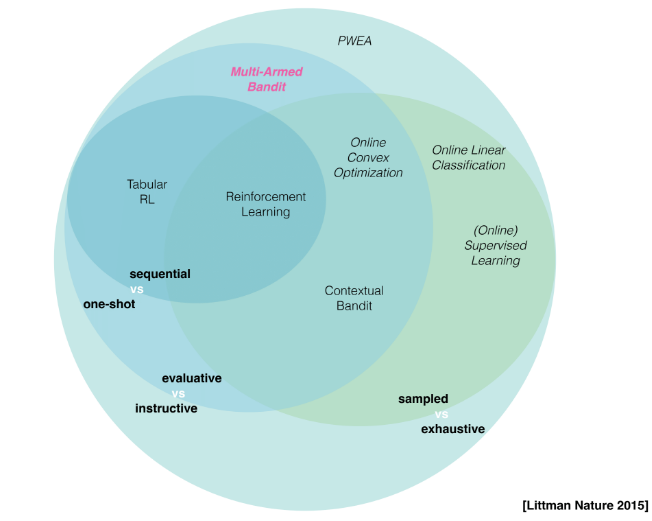
\includegraphics[width=0.75\linewidth]{images/MAB_round.png}
    \caption{Concept venn diagram with Multi-Arm bandits}
    \label{fig:MAB_round}
\end{figure}

\textbf{Why Multi-Arm Bandit ?}
The name comes from imagining a gambler at the slot-machines (also called one arm bandits, because they take away your money!), who has to figure out which machines to play, how many times to play each machine and in which order to play them, and whether to continue with the current machine or try a different machine.

\begin{figure}
    \centering
    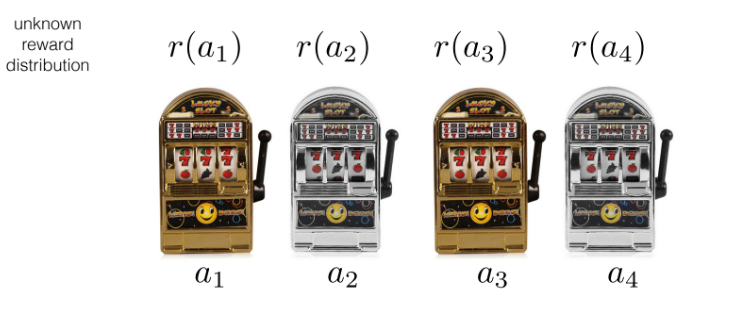
\includegraphics[width=0.75\linewidth]{images/multi_arm_bandit_1.png}
    \caption{Multiple One-Arm bandits. Each have an unknown reward distribution and our objective is to maximize the reward when we have T pulls.}
    \label{fig:slot_machines}
\end{figure}

The current setting of Multi - Armed Bandits makes this problem a:
\begin{itemize}
    \item \textbf{One shot feedback} selecting one action leads to only one reward.
    \item \textbf{Exhaustive feedback} actions are limited and you get to pull arms
    \item \textbf{Evaluative feedback} only a sample of the reward is shown (one the one that you pull),
\end{itemize}
\subsubsection{PWEA vs Bandits}

In PWEA, at any given time T we had access to each of the experts losses. Figure \ref{fig:PWEA} shows an example of PWEA at time stamp 3, where the algorithm made a mistake and we know that experts 1, and experts 2 have made a mistake so we can reduce their weight for the next iteration. But, in the case of MAB only know the reward on the bandit that was chosen and not the others. Figure \ref{fig:partial_feed} shows a example of this.

\begin{figure}
    \centering
    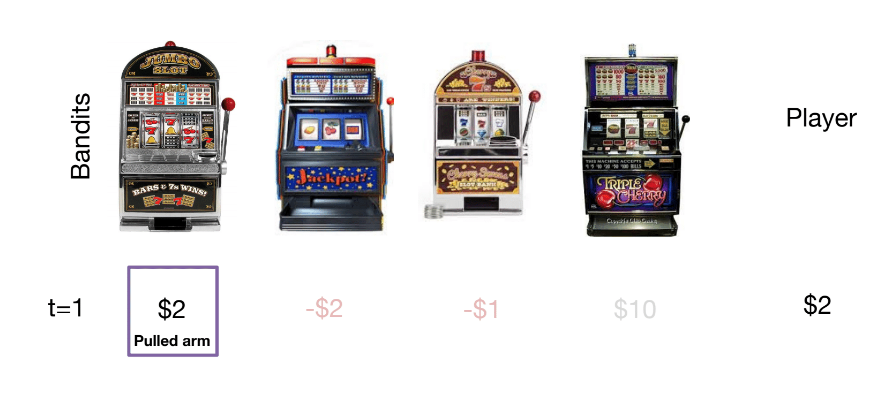
\includegraphics[width=0.75\linewidth]{images/partial_fedback.png}
    \caption{Partial feedback in case of MAB. We cant see the rewards of the bandits whos arm want pulled.}
    \label{fig:partial_feed}
\end{figure}

\textbf{Loss vs Reward} 

Previously we used loss $l \; \in [0,1] \;$ to describe the performance of an algorithm. Similarly we can also define reward $g = 1 - l \; \in [0,1] \;$ to describe the algorithms performance. The objective here would be to maximize this reward. The terms loss and reward can be used interchangeably in the sense that we want to minimize loss or maximize reward for an algorithm. The Regret can also be written in terms of reward:
\begin{align*}
    R^{T}(h) = \underbrace{\sum_{t=1}^{T}g(h(x^T), y^T)}_{\textit{reward of the expert}}-\underbrace{\sum_{t=1}^{T}g(\hat{y}^T, y^T)}_{\textit{reward of the algorithm}}
\end{align*}

\begin{figure}
    \centering
    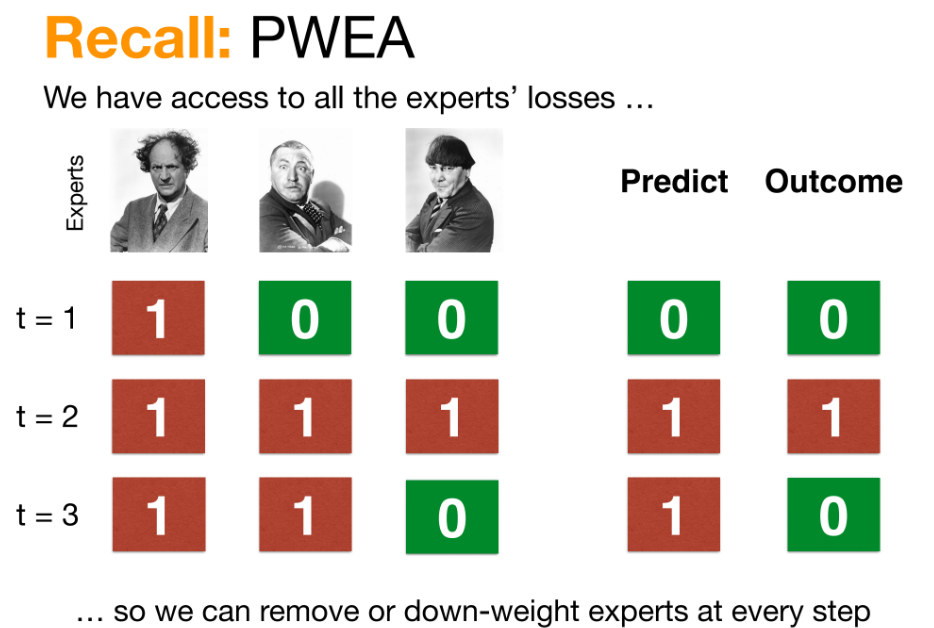
\includegraphics[width=0.75\linewidth]{images/PWEA_recall.png}
    \caption{Classic PWEA, where we have access to all of the experts' losses }
    \label{fig:PWEA}
\end{figure}

\subsubsection{“Exploration and Exploitation” trade-off}

As discussed before that MAB differs from PWEA in the observability of loss. Since we only see the rewards of the arms that were pulled, we need to find balance between 1) exploiting arms that did well in the past, 2) exploring arms that might do well in the future. In PWEA we need not explore because at every instance we can see the loss of other experts. This step of exploration is necessary in case of MAB because we have some/no information about some arms.   
\subsubsection{Applications of Bandits}

\begin{itemize}
    \item \textbf{Which advertisement to display} Suppose you are an advertiser seeking to optimize which ads to show visitors on a particular website. For each visitor, you can choose one out of a collection of ads, and your goal is to maximize the number of clicks over time. The way to think about this in our example is that each ad has some theoretical — but unknown — click-through-rate (CTR) that is assumed to not change over time. How do we go about solving which ad we should choose? \footnote{https://www.spotx.tv/resources/blog/developer-blog/introduction-to-multi-armed-bandits-with-applications-in-digital-advertising/}
    \item \textbf{Robotic grasps} In this senario we consider the  different trajectories (N) the robot can take to be like the N bandits and the reward in this case is if the robot could actually grasp the object or not. 
    \item \textbf{Medical Treatment} MABs can be used in various situations such as to decide the optimal dosage for patients like the authors of \cite{aziz2021multi} suggest, to deciding the course of the medical treatment for a patient \footnote{https://www.ima.umn.edu/materials/2017-2018.4/W9.14-16.17/26479/bandit\_slides\_IMA\_2017.pdf}
    \item \textbf{Packet routing} The authors of \cite{talebi2017stochastic} study online shortest path routing over multi-hop networks, where time-varying link costs or delays are modelled as independent and identically distributed random processes, whose parameters are initially unknown.
    \item \textbf{AI for Go} Alpha Go which is deep-mind's AI for playing Go  simply combined the previous state of the art (Monte Carlo Tree Search [technique inspired from multi-armed bandits]) with the new deep learning techniques.
\end{itemize}
\subsubsection{Types of Bandits}
\begin{itemize}
    \item Stochastic MABs: In this setting, each arm k $\in$ [n] is associated with an (unknown) probability distribution $v_k$ on [0, 1] with true mean $\mu_{k}$, and rewards from arm k are assumed to be drawn i.i.d. from $v_k$.
\item Adversarial MABs: Here there are no probabilistic assumptions on the rewards. Instead, the rewards can be generated by an adversary.
\item Markovian MABs: Here the rewards of each arm follow a Markov process on some underlying state space. The tools used to analyze Markovian MABs are quite different from those used to analyze stochastic and adversarial MABs, and are more similar to tools used in reinforcement learning.
\end{itemize}  


%\section*{References}
%Include your references here. Please cite any resources you found useful.	
%Populate the refs.bib file or list your references manually. Be consistent in formatting!
{
\bibliography{refs}
\bibliographystyle{abbrv}
}

\section{Appendix}
%This section provides any relevant background material that was not covered in the lectures, but was found to be useful for understanding the material. 
%For example, derivations, theory underlying techniques employed, etc.

\subsection{More Applications of MAB}
A comprehensive study of the applications of MAB are nicely mentioned in \cite{bouneffouf2019survey}. A few selected uses cases are mentioned below.

\textbf{Crowdsourcing:} Crowdsourcing has emerged as a powerful means available to employers or service requester to get tasks completed in a timely and cost-effective manner\cite{medium_abhishek}. The employer’s aim is to maximize the number of the tasks completed. The available workers(or employees or freelancers) act as arms in this case, having hidden qualities unknown to the employer. So the problem can be posed as a MAB problem where the employer can either explore the arms to learn their qualities or choose to exploit the best arm identified till now.
%Additionally, this section can summarizes applications or extensions of these techniques found in the literature. 

\textbf{Recommend courses to learners}

MABs are also used in recommending courses to learners in e-learning systems. There are N courses that the e-learning system can recommend to learner. Each course has an unknown rate of success $pi$. $ai$ and $bi$ is the historical number of success (number of learners that finished the course) and failure (number of learners that dropped the course). Each course i is considered to be an arm of a multi-armed bandit with $ai$ success and $bi$ failure. This is a MAB with Bernoulli process and the optimal solution is the Gittins index \cite{whittle1980multi}.

\textbf{Anomaly Detection}

Performing anomaly detection on attributed networks concerns with finding nodes whose behaviors deviate significantly from the majority of nodes. Authors in \cite{ding2019deep} investigate the problem of anomaly detection in an interactive setting by allowing the system to proactively communicate with the human expert in making a limited number of queries about ground truth anomalies. Their objective is to maximize the true anomalies presented to the human expert after a given budget is used up.

\textbf{Bandits for Clustering}

\cite{sublime2018collaborative} considers collaborative clustering, which is machine-learning paradigm concerned with the unsupervised analysis of complex multiview data using several algorithms working together. The authors propose a collaborative peer to peer clustering algorithm based on the principle of non stochastic multi-arm bandits to assess in real time which algorithms or views can bring useful information.

\textbf{Finance}

In recent years, sequential portfolio selection has been a focus of increasing interest at the intersection of the machine learning and quantitative finance. The trade-off between exploration and exploitation, with the goal of maximizing cumulative reward, is a natural formulation of the portfolio choice problems. In \cite{shen2015portfolio}, the
authors proposed a bandit algorithm for making online portfolio choices via exploiting correlations among multiple arms. In \cite{huo2017risk}, the authors incorporate risk-awareness into the classic multi-armed bandit setting and introduce a novel algorithm for portfolio construction. Through filtering assets based on the topological structure of financial market and combining the optimal multi-armed bandit policy with the minimization of a coherent risk measure, they achieve a balance between risk and return.
\end{document} % Done!Exercise scheduling
